%chapter introduce un nuevo cap�tulo
\chapter{Desarrollo}

Este proyecto de resume en.................

\section{Plataforma rob�tica}

El primer paso para la realizaci�n de este proyecto fue el estudio y selecci�n de las plataformas rob�ticas que pueden conseguirse actualmente. Dado que el objetivo es encontrar un robot humanoide sobre el que se pueda implantar un sistema de visi�n, es necesario analizar diversos aspectos; algunos mec�nicos como el numero y fuerza de los actuadores, y otros electr�nicos como la capacidad de procesamiento y velocidad del controlador. Sin embargo, dado que este proyecto es autofinanciado en su mayor medida, el factor econ�mico tambi�n es un limitante destacable. 

A continuaci�n se presenta un estudio las principales principales opciones.

\subsection{Selecci�n de una plataforma rob�tica}

En el mercado existe una gran variedad de robots educativos que cumplen las caracter�sticas antropom�rficas necesarias para ser considerados robots mini-humanoides. Los robots que se muestran a continuaci�n son una recopilaci�n de algunos de los modelos mas accesibles y extendidos.

\subsubsection{Robonova, de Hitec}

El Robonova (figura \ref{robonova}) es uno de los mini-humanoides mas extendidos a nivel mundial. Fue uno de los primeros robots de este tipo que se fabric� comercialmente y marc� un antes y un despues en su categor�a. Es por esto que es muy com�n encontrar Robonovas en competiciones como Ceabot, ya que durante muchos a�os fue el robot mini-humanoide mejor equipado y mas vendido. En la Asociaci�n de Rob�tica de la Universidad Carlos III, se han utilizado Robonovas en competiciones y proyectos desde su fundaci�n.

\begin{figure}[h]
\centering
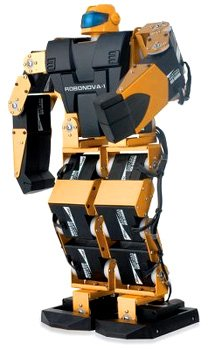
\includegraphics[width=0.4\textwidth]{figuras/robonova}   
\caption{Robonova, de Hitec}
\label{robonova}
\end{figure}

El kit de f�brica cuenta con 16 grados de libertad. Sus actuadores son servos digitales HSR 8498HB, que desarrollan un torque de 7.4kg/cm. Cabe destacar de estor servos su funci�n "Motion Feedback", es decir, su capacidad para leer posiciones y comunicarselas al controlador.
La placa de control del Robonova est� basada en un microcontrolador ATMega 128 y cuenta con hasta 40 pines GPIO (puertos binarios de entrada y salida), 8 entradas anal�gicas, 3 salidas PWM, puerto serie y conexi�n I2C. Gracias a esto, el Robonova es f�cilmente ampliable con sensores y actuadores, no necesariamente de la misma marca. En cuanto al software, Hitec da soporte a la programaci�n con RoboBasic, un entorno de desarrollo completo con un lenguaje basado en Basic. 

\subsubsection{KHR-3HV, de Kondo}

El KHR-3HV (figura \ref{kondo}), del fabricante japon�s Kondo, es uno de los mini-humanoides mas avanzados actualmente. Puede presumir de ser el modelo de serie mas utilizado en el campeonato Robo-One, siendo seleccionado por los equipos por su gran agilidad y tama�o compacto.

\begin{figure}[h]
\centering
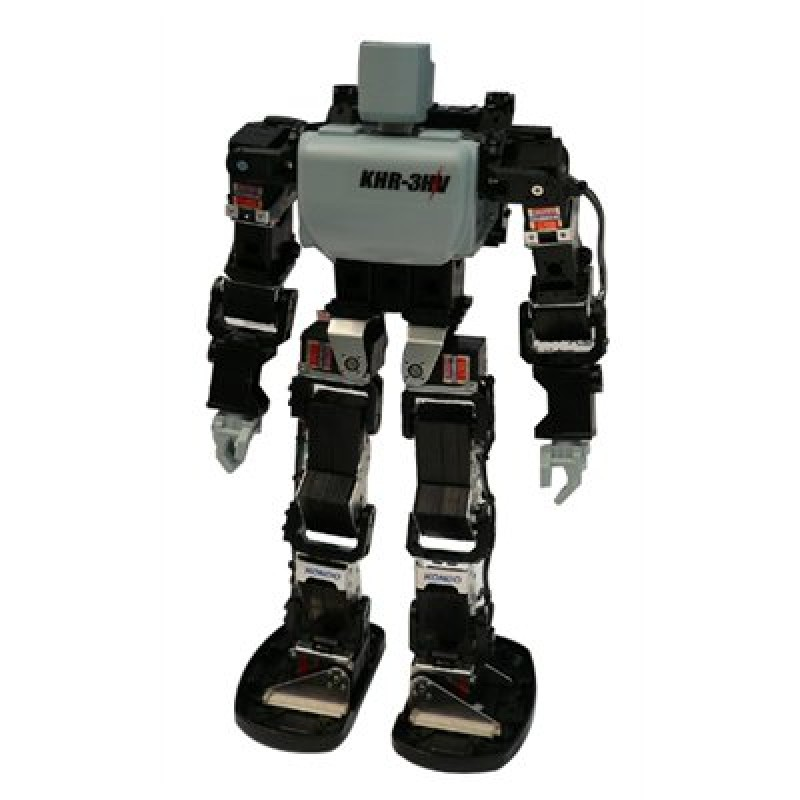
\includegraphics[width=0.8\textwidth]{figuras/kondo}   
\caption{KHR3-HV, de Kondo}
\label{kondo}
\end{figure}

En su configuraci�n standard, el KHR-3HV cuenta con 17 servomotores KRS-2552HV de 14kg/cm de torque. Dichos actuadores, adem�s, incluyen un peque�o microcontrolador, lo que les permite conectarse en daisy chain. El robot incluye una controladora RCB-4, expandible con 10 entradas analogicas y 10 GPIOs, y con capacidad para controlar hasta 35 servos. El software de programaci�n ofrecido por Kondo es el Heart to Heart V4, que puede ser descargado gratuitamente desde su web oficial. Es importante recalcar que gracias a su inmensa comunidad de usuarios, existen varios proyectos de c�digo abierto con librer�as que permiten programar el KHR-3HV en lenguajes mas convencionales, como C y Python.

\subsubsection{5710k, de RoboBuilder}

Uno de los robots mas interesantes por su at�pica configuraci�n de servomotores es el RoboBuilder 5710k. Se presenta como un kit modular con el que se pueden construir diferentes configuraciones de robots, sido la mas "avanzada" la antropom�rfica.


\subsubsection{Robovie-X, de Vstone}
The Robovie-X is the standard model and comes with 17 degrees of freedom and features VS-S092J servos which have 9.2kg/cm of torque. The VS-RC003HV onboard controller features a built-in audio system.
\subsubsection{Bioloid, de Robotis}









\section{Modificaciones sobre el robot Bioloid}


\paragraph{Palabras clave:} palabraclave1, palabraclave2, palabraclave3.

